\documentclass{beamer}
\usepackage{tikz}

% internal parameters
\usetheme{Copenhagen}
\usecolortheme{default}
\setbeamertemplate{caption}[numbered]

% packages
\usepackage{graphics}
\usepackage{amsmath}
\usepackage{xcolor}
\usepackage{physics}
\usepackage{fontawesome}
\usepackage{mathrsfs}  
\usepackage{multirow}
% \usefonttheme{professionalfonts}


\title[Wobbling Motion]{New Results Concerning Collective Motion in Triaxial Nuclei}
\author[Robert POENARU]{Robert POENARU\inst{1,2}}

\institute[VFU]
{
  \inst{1}%
  Doctoral School of Physics @ UB\\
  Bucharest, Romania
  \and
  \inst{2}%
  Dept. of Th. Phys. @ IFIN-HH\\
  Magurele, Romania
}

\date{\textit{UB Faculty of Physics Meeting}\\\textit{\today}}

%------------------------------------------------------------
%The next block of commands puts the table of contents at the 
%beginning of each section and highlights the current section:
% \AtBeginSection[]
% {
%   \begin{frame}
%     \frametitle{Table of Contents}
%     \tableofcontents[currentsection]
%   \end{frame}
% }

%------------------------------------------------------------
\begin{document}
%---------------------------------------------------------
\frame{\titlepage}
% \begin{frame}
%   \frametitle{Table of Contents}
%   \tableofcontents
% \end{frame}

\begin{frame}{Nuclear Deformation}
\par Most of the nuclei are either \emph{spherical} or \emph{axially symmetric} in their ground-state.
\par Deformation parameter $\beta$ (\textit{Bohr, 1969}): preserves axial symmetry
\begin{figure}
  \centering
  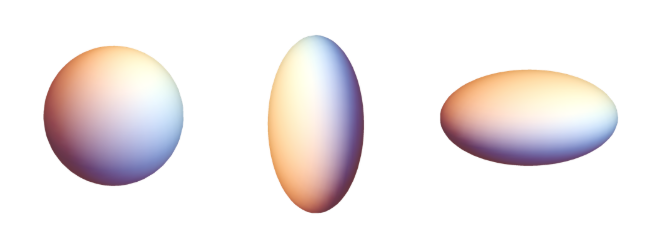
\includegraphics[width=0.99\textwidth]{Figs/nuclear_shapes.png}
  \caption{\textbf{spherical:} $\beta=0$\ \textbf{prolate:} $\beta>0$\ \textbf{oblate:} $\beta<0$}
\end{figure}
\end{frame}

\begin{frame}
  \frametitle{Nuclear Triaxiality}
  \begin{alertblock}{Non-axial shape}
    \par Deviations from symmetric shapes can occur across the chart of nuclides $\to$ \textbf{triaxial nuclei}.
    \par The triaxiality parameter $\gamma$ (\textit{Bohr, 1969}): departure from axial symmetry
  \end{alertblock}
  \begin{figure}
    \centering
    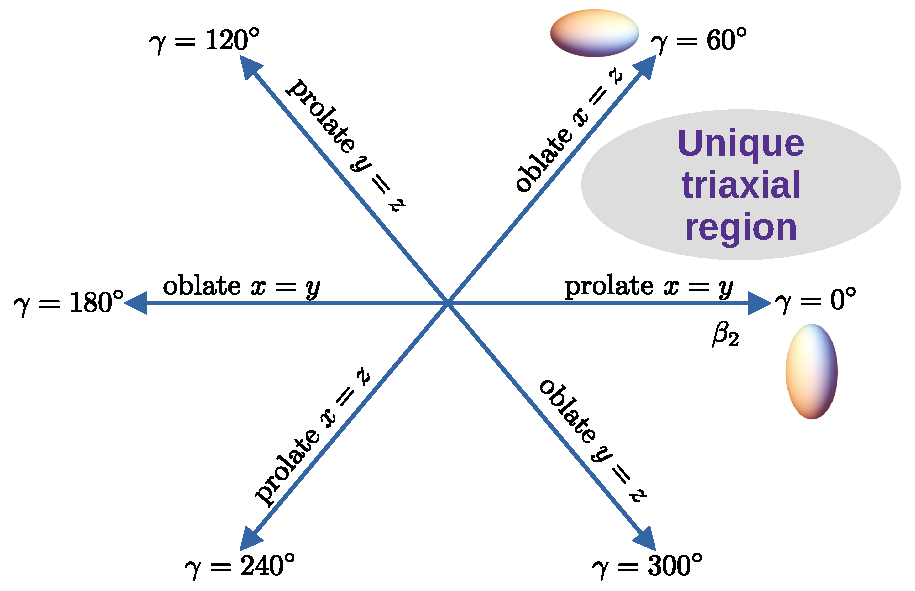
\includegraphics[scale=0.42]{Figs/nice_diagram.pdf}
    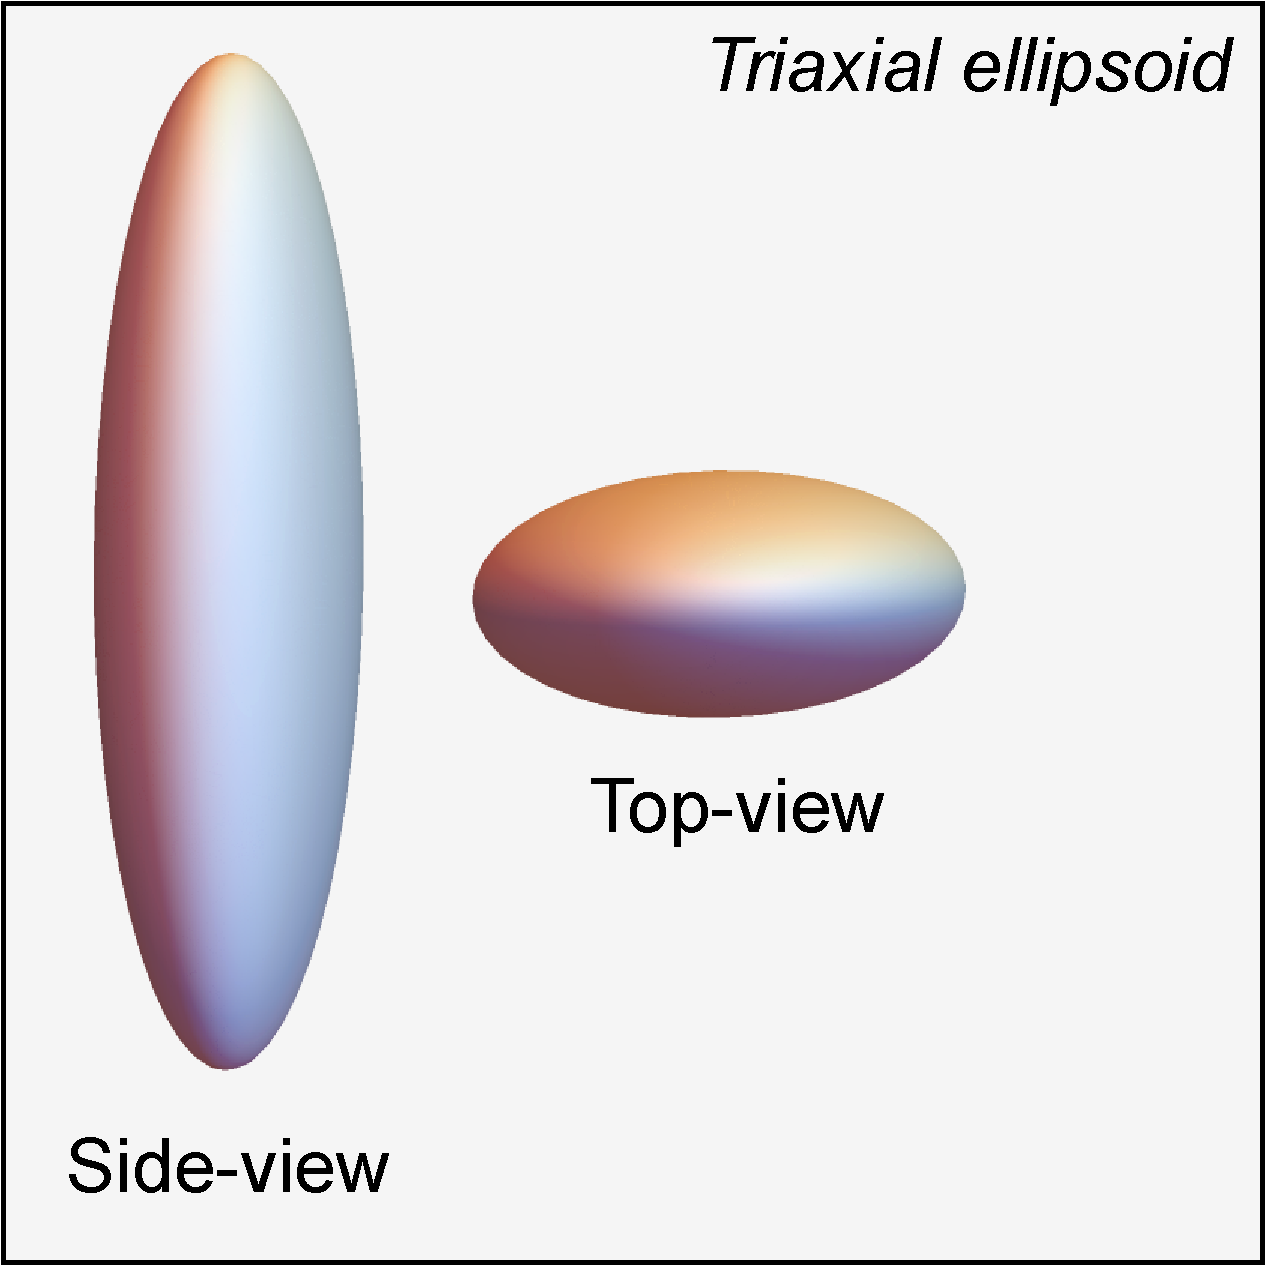
\includegraphics[scale=0.19]{Figs/triaxial-shape.pdf}
    % \caption{The $(\beta,\gamma)$ plane divided into six equivalent parts, depicting nuclear surfaces.}
  \end{figure}
\end{frame}

\begin{frame}
  \frametitle{Fingerprints for Triaxiality}
  \begin{itemize}
    \item Stable triaxial nuclei represent a real challenge
    \item Clear signatures for confirming stable triaxiality in nuclei
    \begin{enumerate}
      \item Chiral symmetry breaking (\textit{Frauendorf, 1997})
      \item \textbf{Wobbling motion} (\textit{Bohr \& Mottelson, 1975})
    \end{enumerate}
  \end{itemize}
  \begin{block}{Wobbling Motion (WM)}
    \begin{itemize}
      \item Unique to non-axial nuclei
      \item Predicted 50 years ago for even-$A$ nuclei
      \item First experimental evidence for $^{163}$Lu (\textit{Ødegård}, 2001)
      \item Currently: confirmed wobblers within the mass regions $A\approx[100,130,160,180]$.
    \end{itemize}
  \end{block}
\end{frame}

% \begin{frame}
%   \frametitle{Energy of Deformed Nuclei}
%     \begin{block}{Collective Motion}
%       \begin{itemize}
%         \item A nucleus - \emph{droplet} - can generate angular momentum from the rotation and vibration of the droplet itself
%         \item Each individual nucleon contributes to the total angular momentum $\rightarrow$ \emph{collectiveness}
%         \item \faWarning Rotation can occur only if the nuclear potential is \emph{deformed}
%       \end{itemize}
%     \end{block}
%     \begin{figure}
%       \centering
%       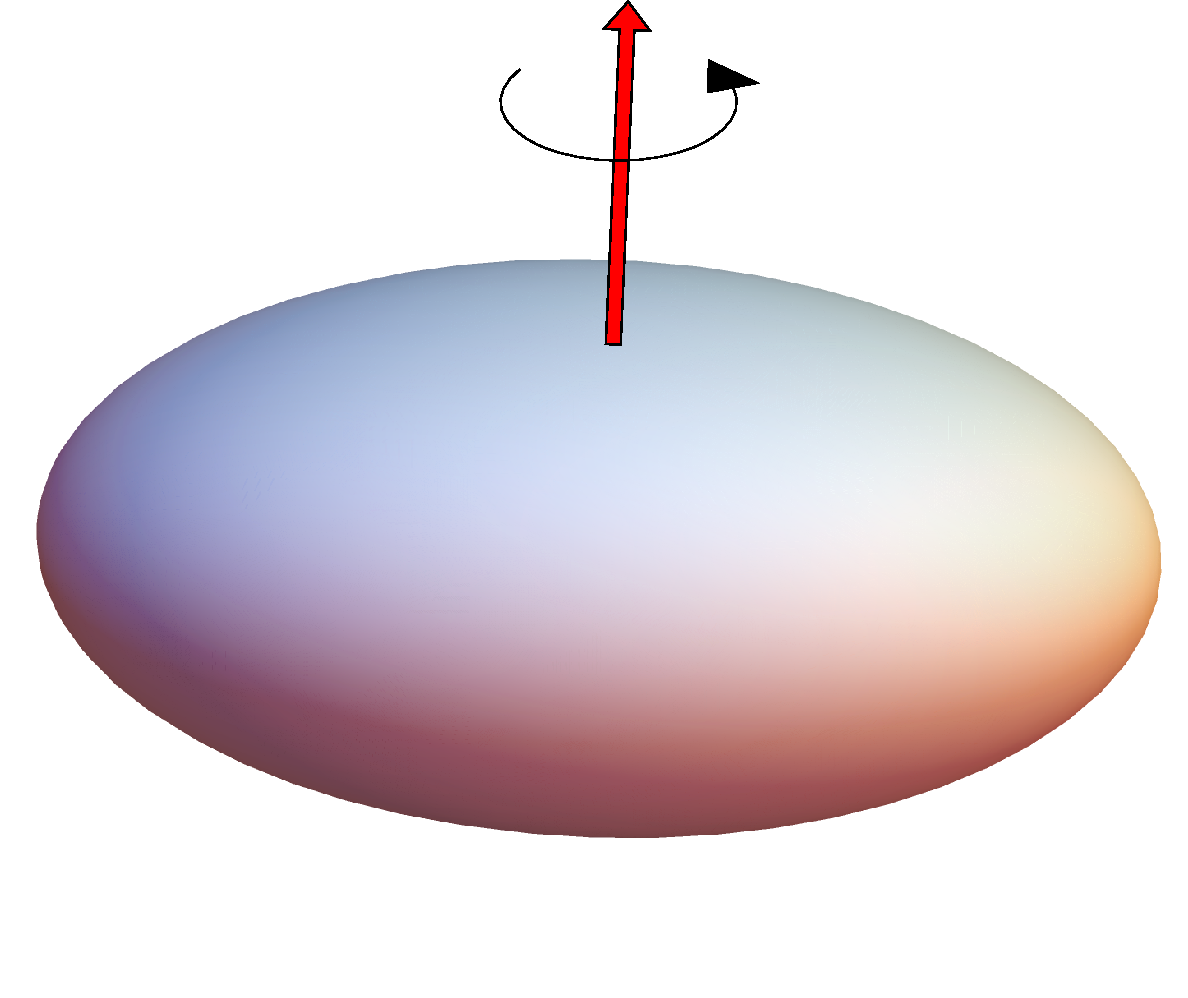
\includegraphics[scale=0.2]{Figs/collective-rotation.pdf}
%     \end{figure}
% \end{frame}

\begin{frame}
  \frametitle{Triaxial Rotor Energy}
  \begin{itemize}
    \item A triaxial nucleus can rotate about any of the three axes
    \item Rotation about the axis with \textbf{the largest moment of inertia} (MOI) is energetically the most favorable: $E_\text{rot}\propto\frac{\hbar^2}{2\mathcal{J}_\text{max}}I(I+1 )$
    \item MOI anisotropy $\rightarrow$ the \emph{main rotation} around $\mathcal{J}_\text{max}$ is disturbed by the other two axes $\rightarrow$ {\color{red}\emph{total motion of the rotating nucleus has an oscillating behavior}}
  \end{itemize}
  \begin{figure}
    \centering
    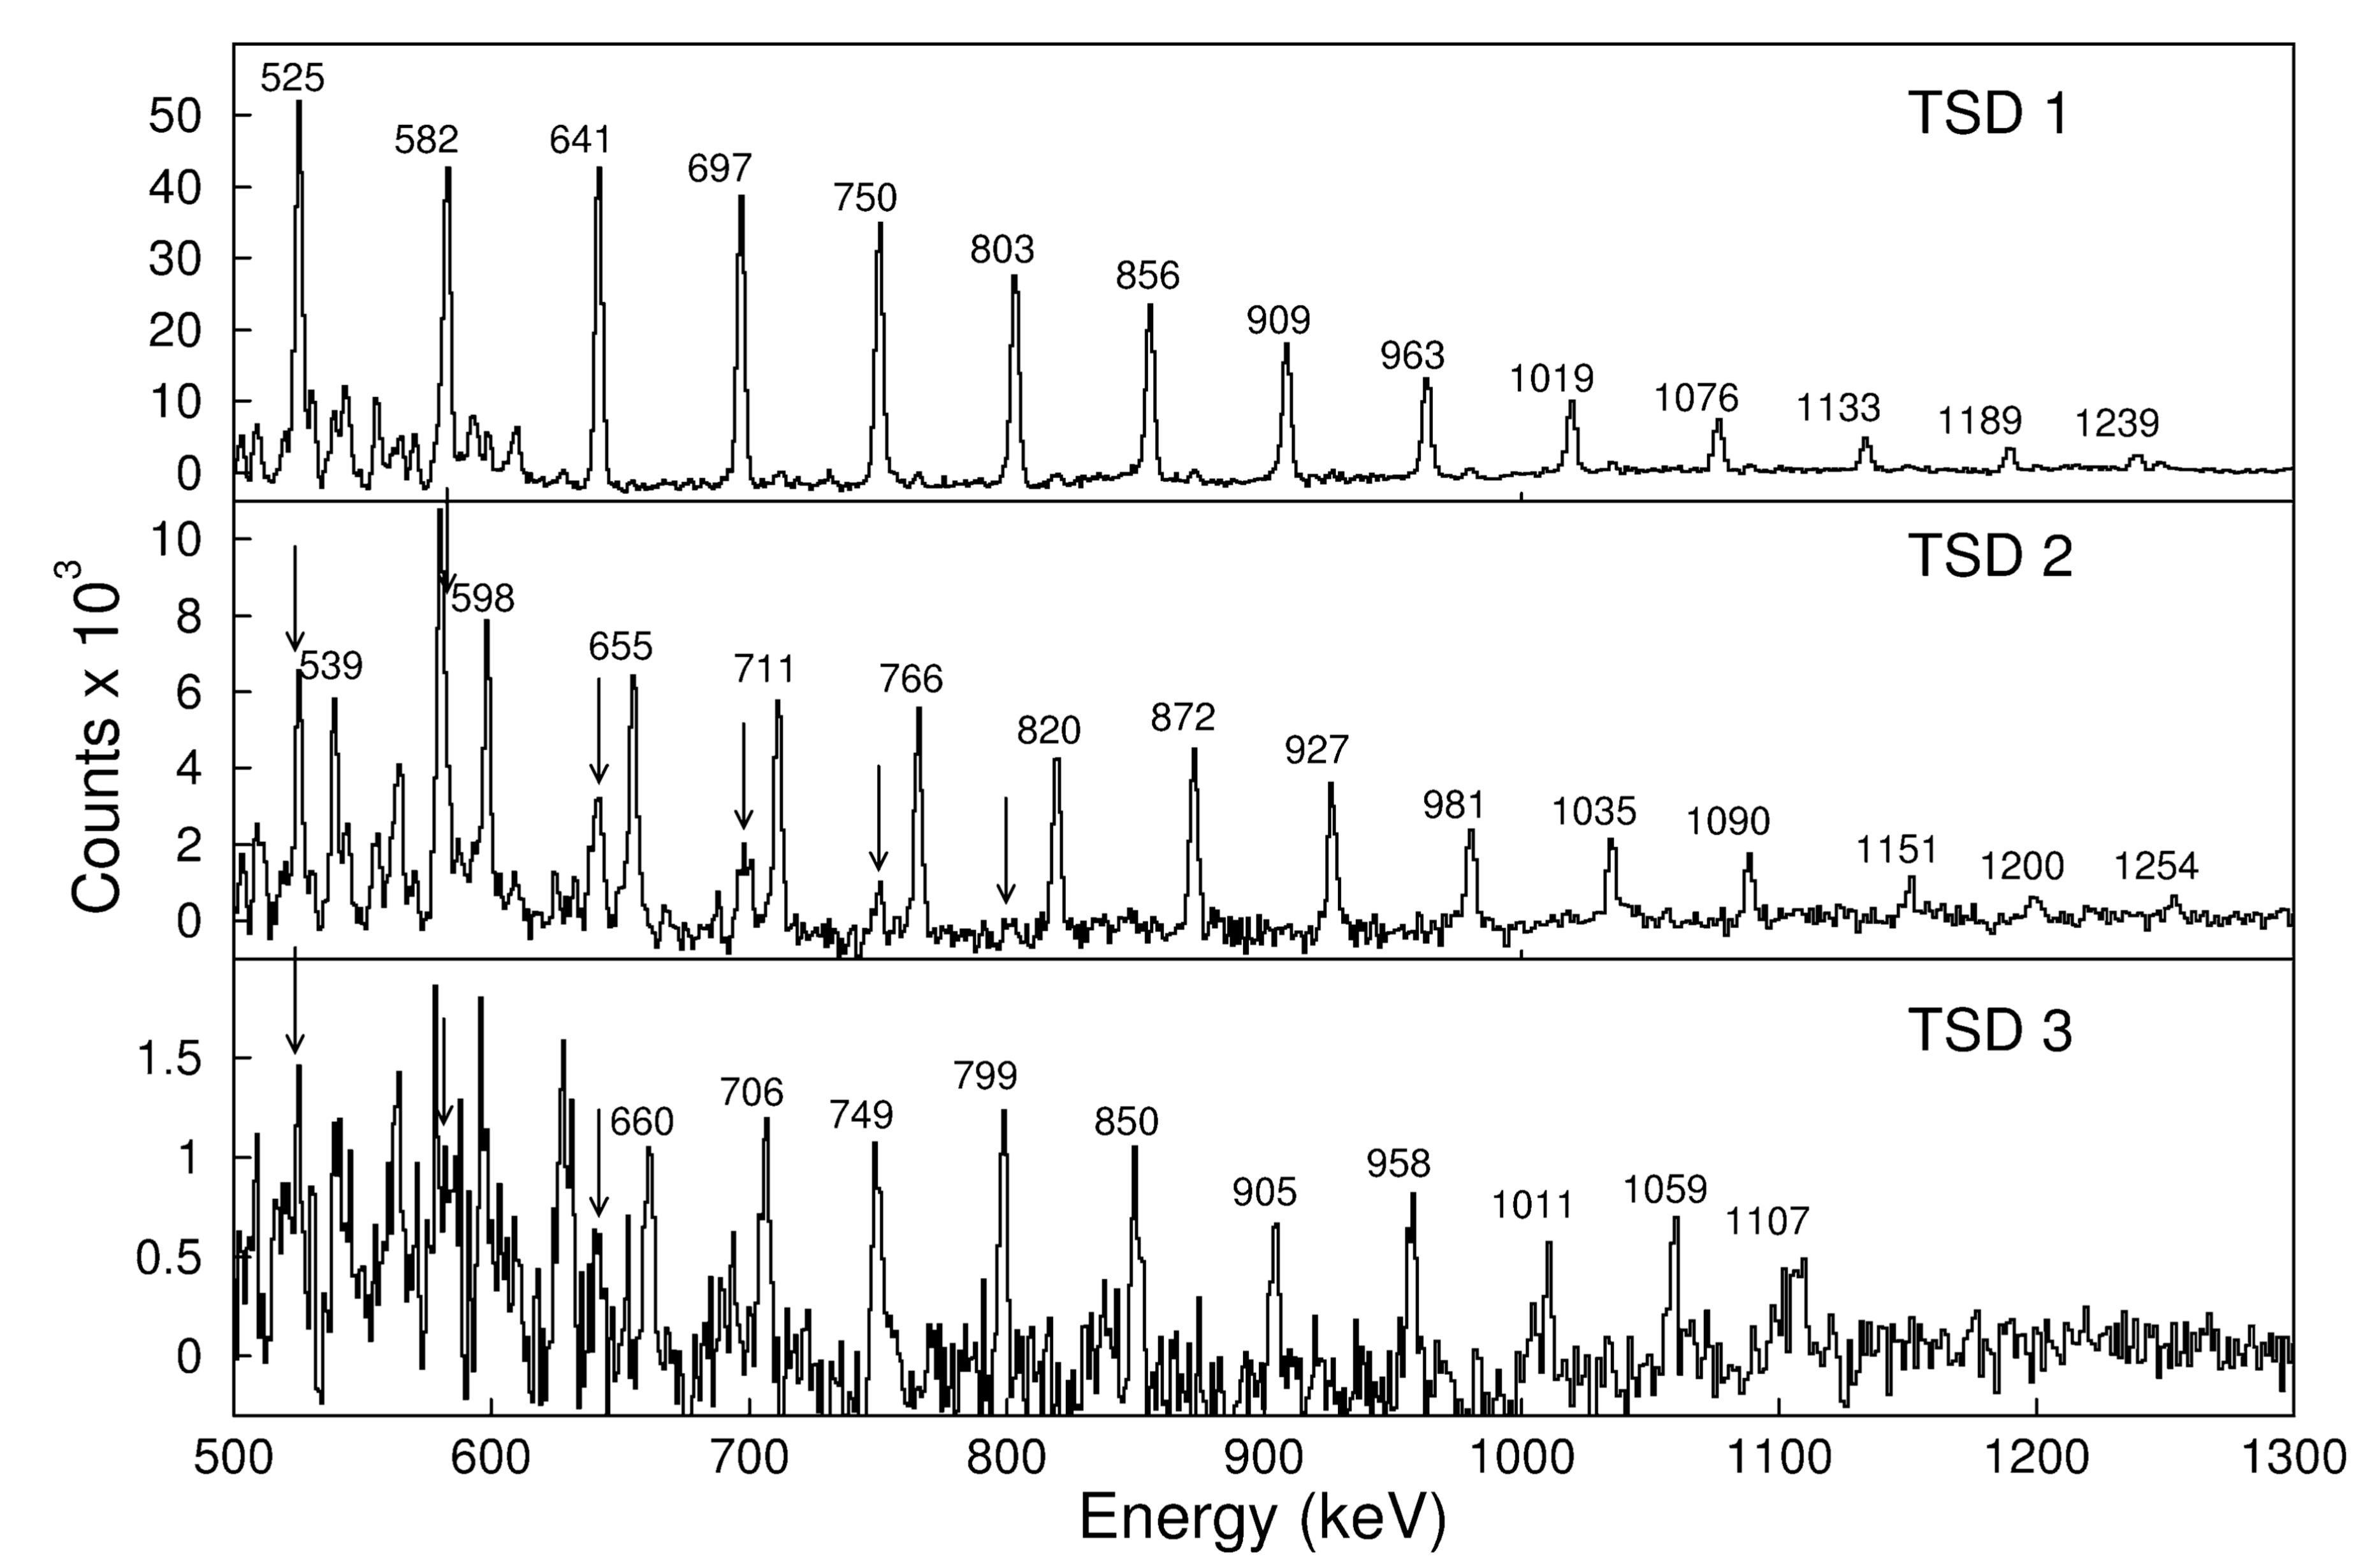
\includegraphics[scale=0.1]{Figs/collective-spectra.pdf}
    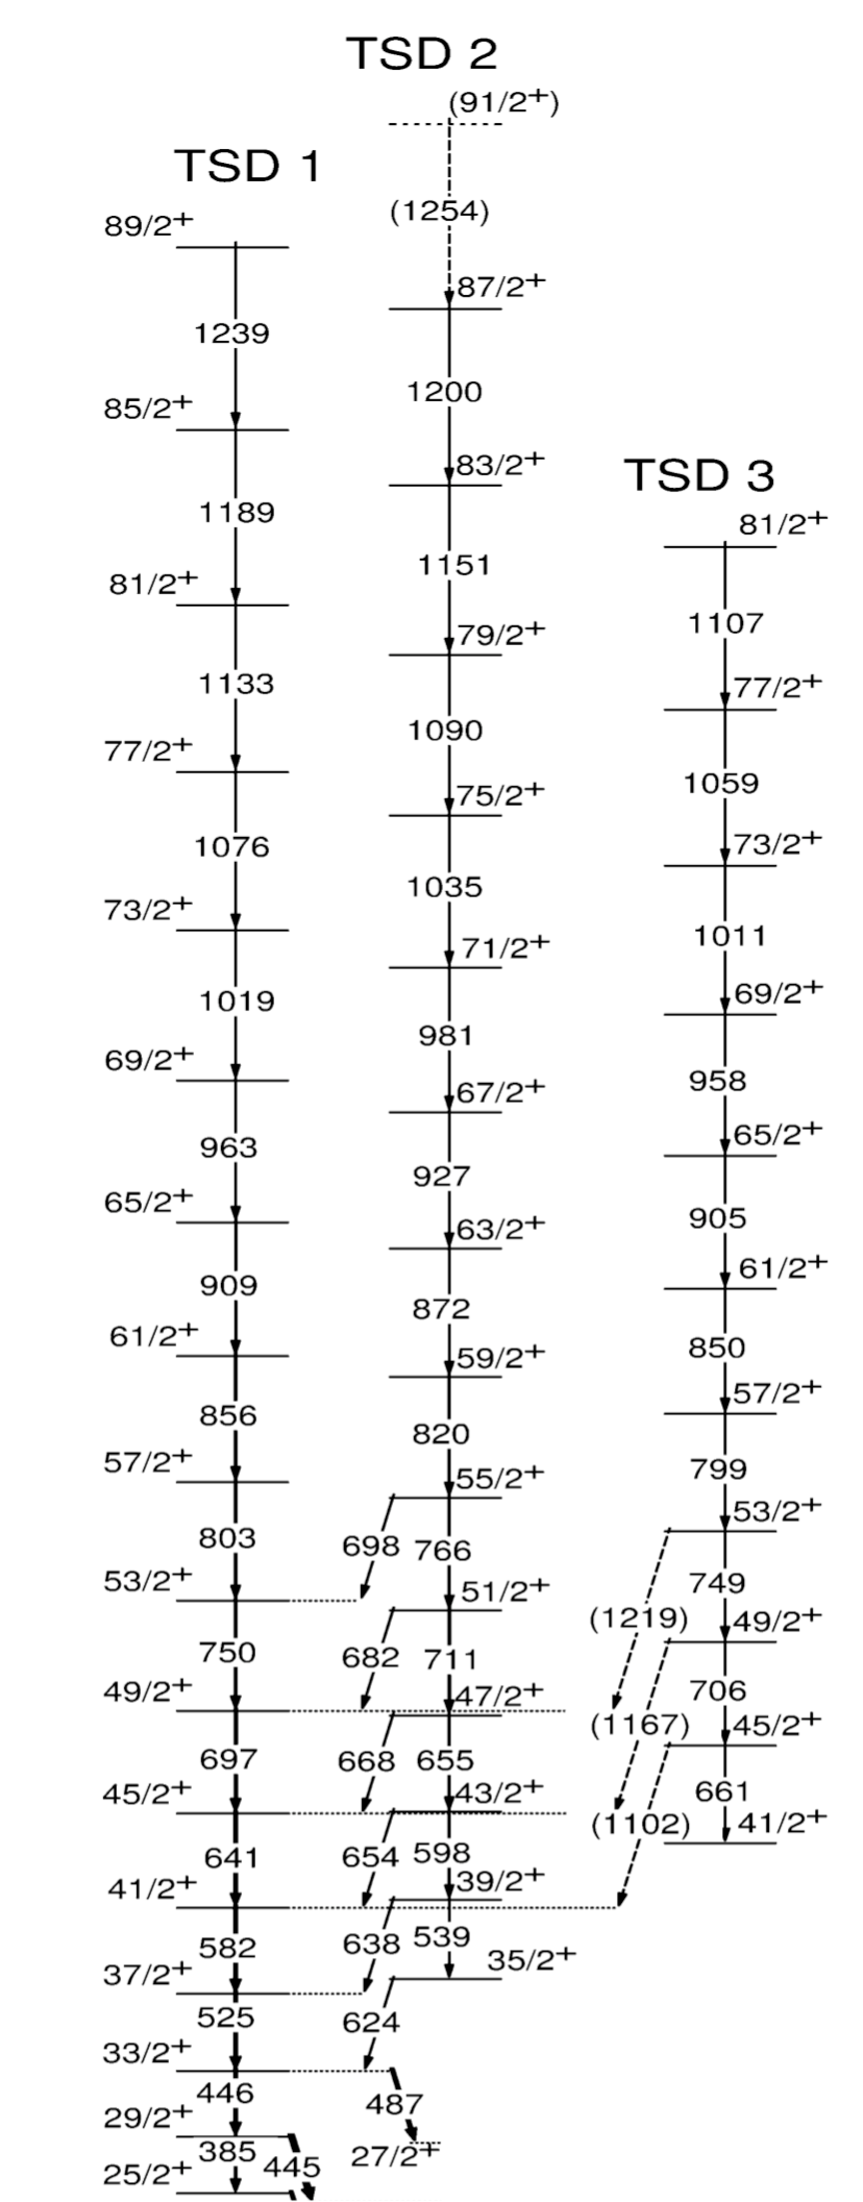
\includegraphics[scale=0.11]{Figs/collective-levels.pdf}
  \end{figure}
  \tiny{\textit{Figures from Schönwaßer et al., 2001}}
\end{frame}

\begin{frame}
  \frametitle{Wobbling Motion}
\begin{itemize}
  \item Total angular momentum $\mathbf{I}$ disaligned w.r.t. body-fixed axes
  \item The a.m. \textbf{precesses} and \textbf{wobbles} around the axis with $\mathcal{J}_\text{max}$
  \item The precession of $\mathbf{I}$ can increase by \textbf{tilting} 
  \item Tilting by an energy quanta $\sim$ \emph{vibrational character} $\rightarrow$ \textbf{wobbling phonon} $n_w=0,1,2...$
\end{itemize}
  \begin{figure}
    \centering
    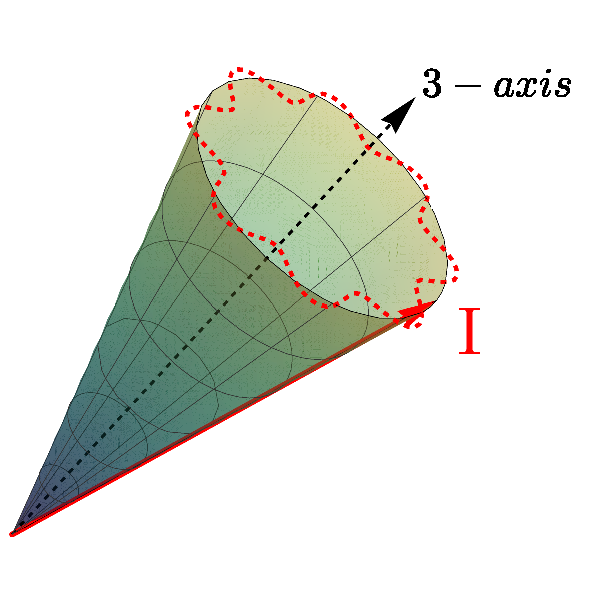
\includegraphics[scale=0.42]{Figs/precessional_cone_2.pdf}
    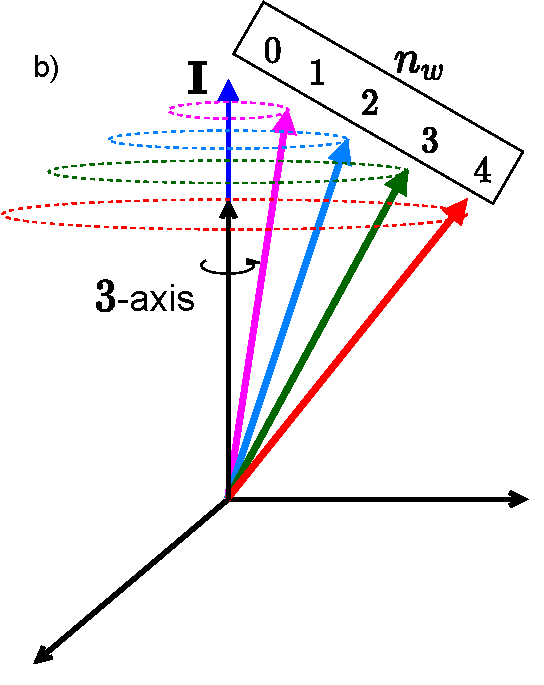
\includegraphics[scale=0.37]{Figs/wobbling_n_schematic-2.pdf}
  \end{figure}
\end{frame}

\begin{frame}
  \frametitle{Wobbling Spectrum}
\begin{block}{Even-$A$ Nuclei}
  \begin{itemize}
    \item Employing the Harmonic Approximation \textit{(Bohr, 1969)}
    \item $\hat{H}$ composed of a {\color{red}\emph{rotational}} part and {\color{blue}\emph{harmonic oscillation}} (i.e., wobbling) part:
  \end{itemize}
  \begin{align}
    \hat{H}={\color{red}\frac{\hbar^2}{2\mathcal{J}_\text{max}}I(I+1)}+{\color{blue}\hbar\omega_\text{wob}\left(n_w+\frac{1}{2}\right)}\ , n_w=0,1,2,\dots
    \label{wobbling-hamiltonian-even-A}
  \end{align}
\end{block}
\begin{figure}
  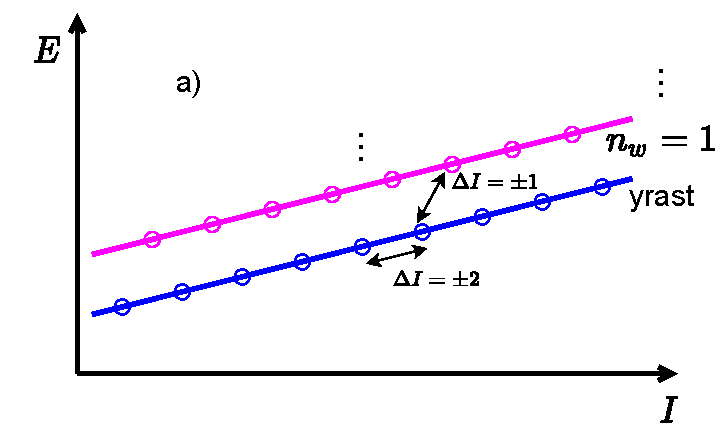
\includegraphics[scale=0.5]{Figs/wobbling_n_schematic-1.pdf}
  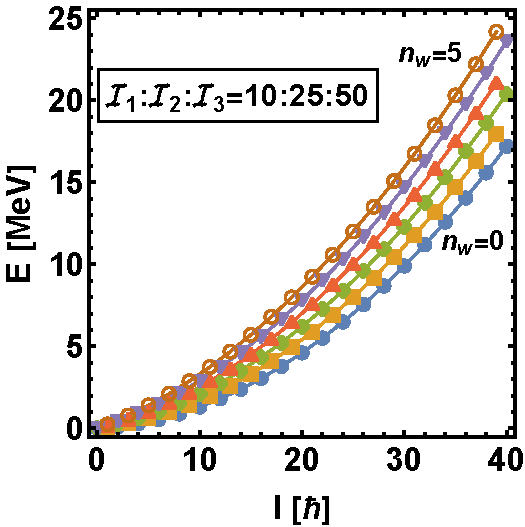
\includegraphics[scale=0.4]{Figs/wobblingFreq-evenA.pdf}
\end{figure}
\end{frame}

\begin{frame}
  \frametitle{New Results for A=130}
  \begin{minipage}{.8\textwidth}
    \begin{block}{Recent findings for even-even nuclei}
      \begin{itemize}
        \item Two wobbling bands have been identified experimentally in \textbf{$^\mathbf{130}$Ba} (\textit{Petrache et al., 2019})
        \item DFT+PRM description of the wobbling motion described the excited spectra (\textit{Chen et al., 2019})
        \item Stable triaxiality for $\beta=0.24$ and $\gamma=21.5^\circ$
        % \item Infer spin-dependence for $\mathcal{J}_{1,2,3}$
      \end{itemize}
    \end{block}
  \end{minipage}%
  \begin{minipage}{.2\textwidth}
    \begin{figure}
      \centering
      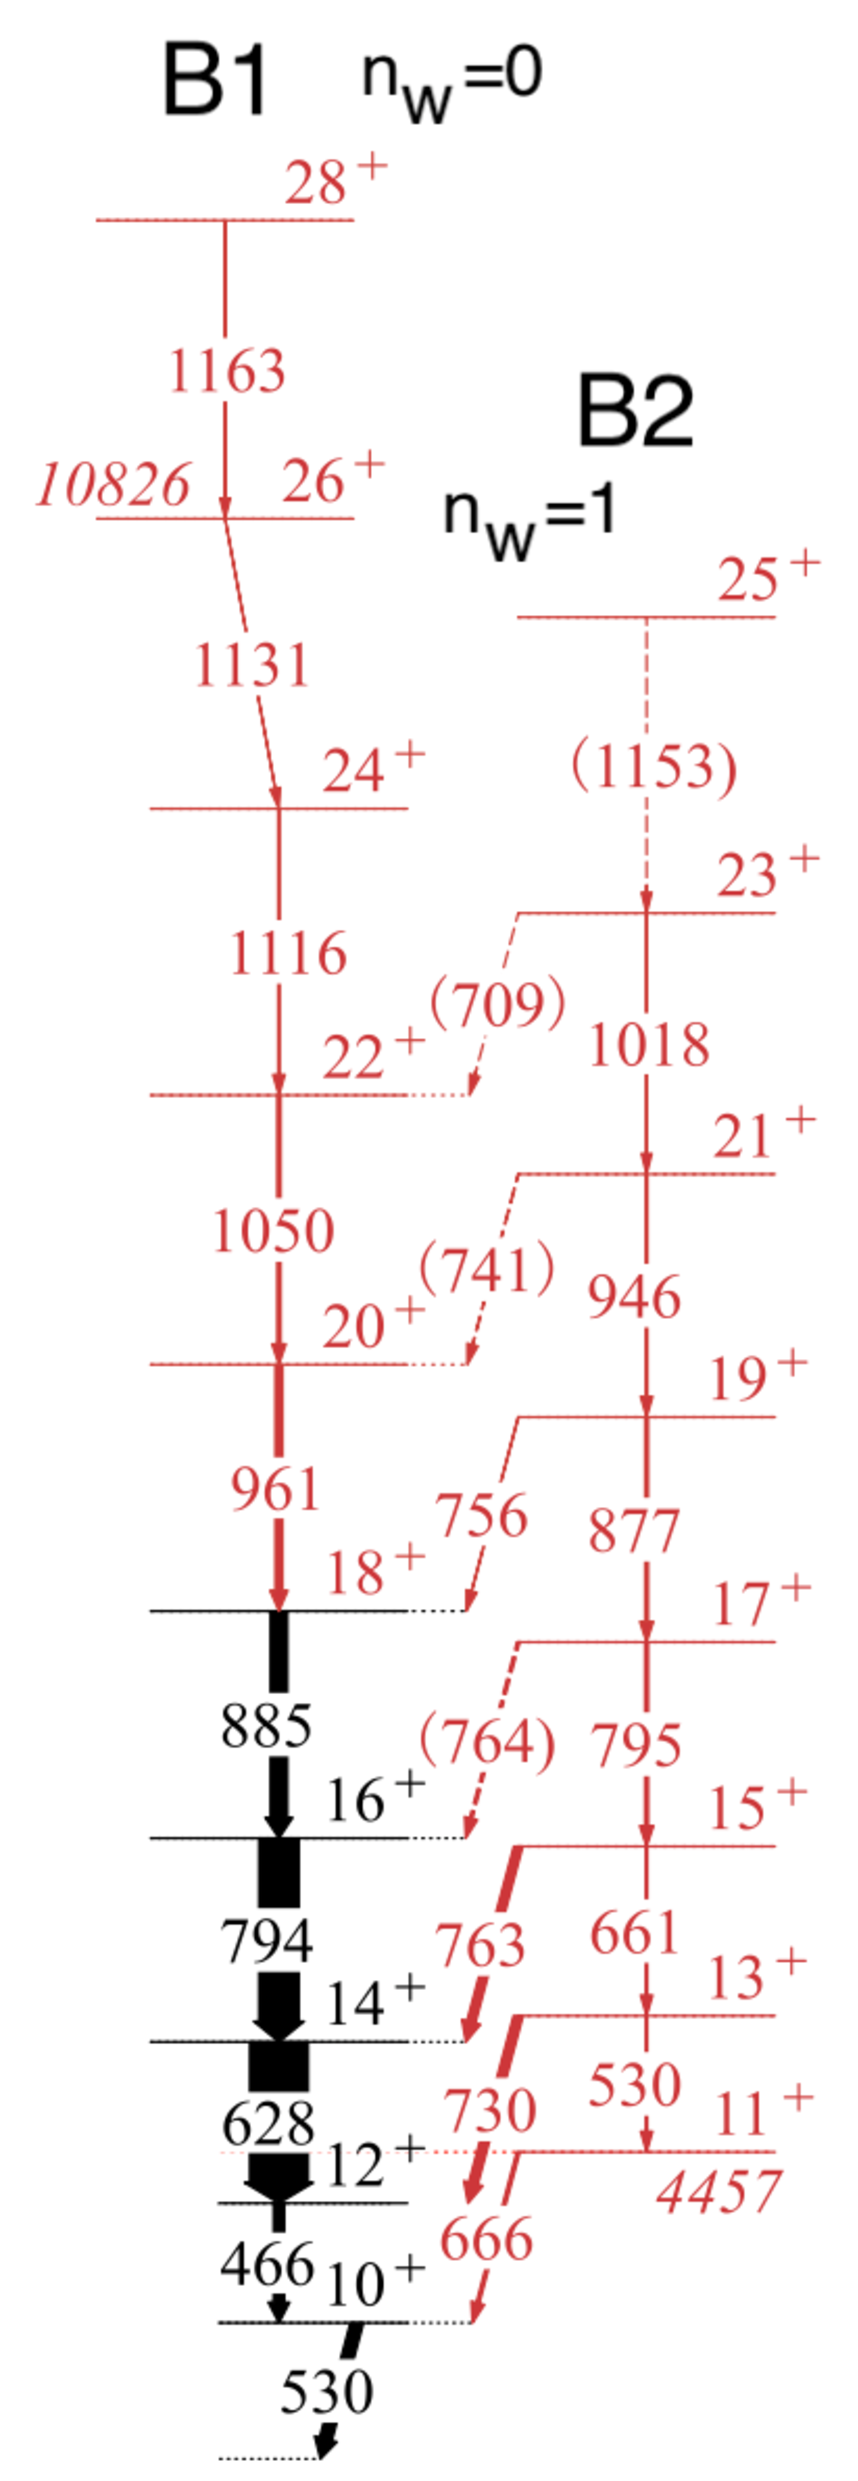
\includegraphics[scale=0.13]{Figs/ba-130-level-scheme.pdf}
      \tiny{\textit{Figure from Petrache et al., 2019}}
    \end{figure}
  \end{minipage}
\end{frame}

\begin{frame}
  \frametitle{New Results for A=130 II}
  \begin{columns}
    \begin{column}{0.65\textwidth}
      % \begin{alertblock}{Harmonic Approximation}
        \begin{itemize}
          \item Employed an energy spectrum of harmonic type according to Eq. \ref{wobbling-hamiltonian-even-A}:
          \begin{align}
            E_{I}={\color{red}\frac{\hbar^2}{2\mathcal{J}_3}I(I+1)}+{\color{blue}\hbar\omega_\text{wob}\left(n_w+\frac{1}{2}\right)}\nonumber
          \end{align}
          \item wobbling frequency - linear dependence on $I$ (fixed MOI ordering $\mathcal{J}_3>\mathcal{J}_{1,2}$)
          \begin{align}
            {\color{blue}\hbar\omega_\text{wob}(I)=2f(\mathcal{J}_1,\mathcal{J}_2,\mathcal{J}_3)\cdot I}\nonumber
          \end{align}
        \end{itemize}
      % \end{alertblock}
    \end{column}
    \begin{column}{0.4\textwidth}
      \begin{figure}
        \begin{center}
          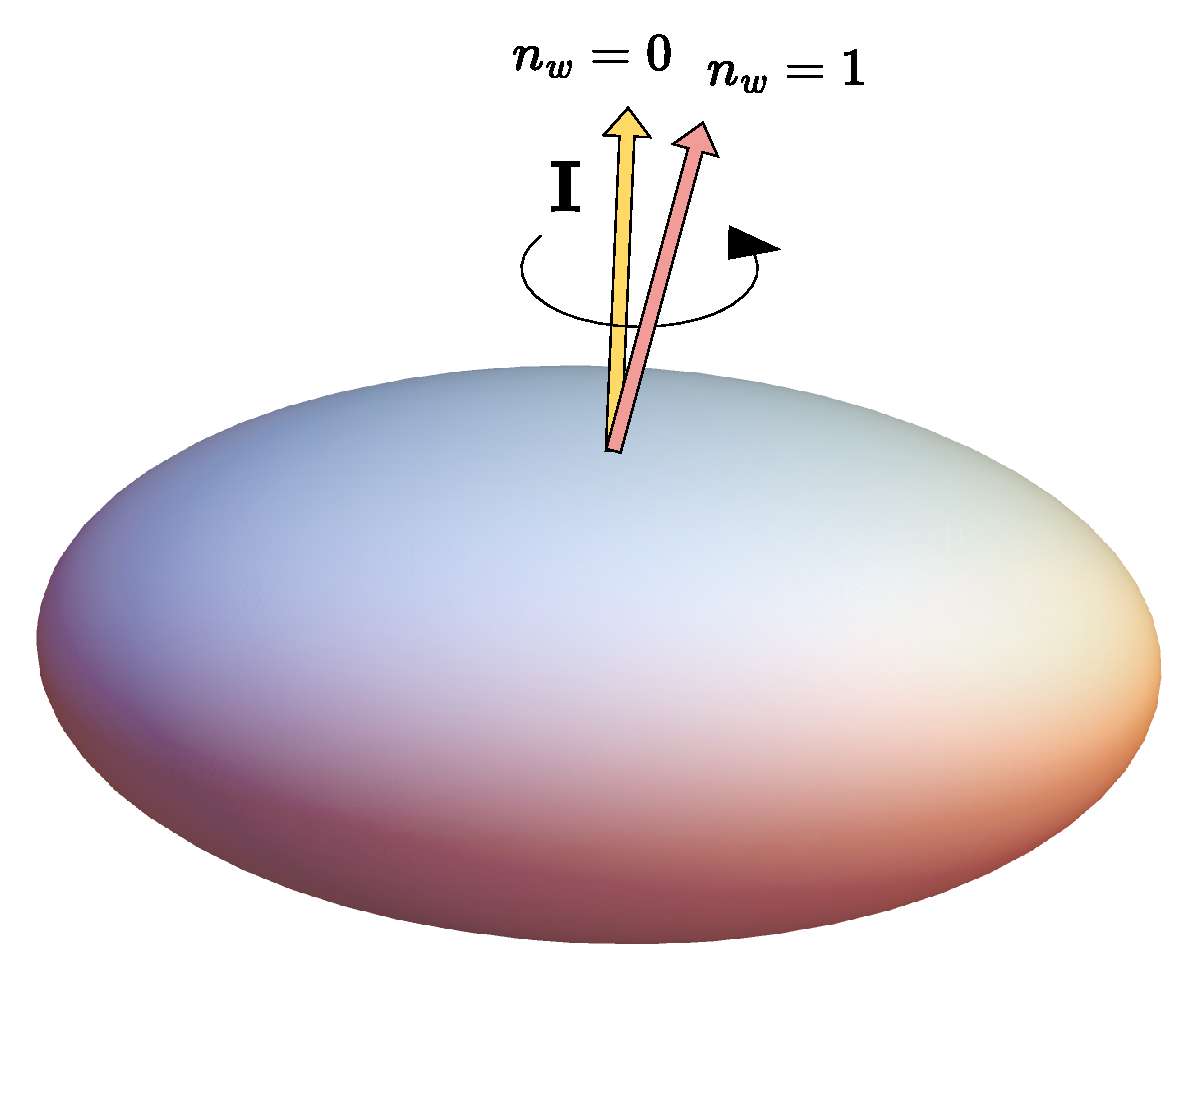
\includegraphics[scale=0.21]{Figs/triaxial-shapes-even-A.pdf}
        \end{center}
      \end{figure}
    \end{column}
  \end{columns}
\end{frame}

\begin{frame}
  \frametitle{New Results for A=130 III}
  \begin{columns}
    \begin{column}{0.75\textwidth}
      \begin{alertblock}{Harmonic Approximation}
        \begin{itemize}
          \item Reproduced the excited spectra for $\{B1,B2\}$
          \item Fix a \emph{free parameter set}: $\mathcal{P}=\left[\mathcal{J}_1,\mathcal{J}_2,\mathcal{J}_3\right]$
          \item Adopt a fitting procedure:
          \begin{align}
            \chi^2=\frac{1}{N_T}\sum_{i=1}^{N_T}\frac{\left(E_\text{exp}^{(i)}-E_\text{th}^{(i)}\right)^2}{E_\text{exp}^{(i)}}
          \end{align}
          % \item $\texttt{min}\left[\chi^2\right]\longrightarrow\mathcal{P}_\text{fit}$.
        \end{itemize}
      \end{alertblock}
      \begin{exampleblock}{Results for $^{130}$Ba \textbf{PRELIMINARY!}}
        \begin{table}
          \centering
          \begin{tabular}{|c|c|c|c|}
          \hline
          $\mathcal{J}_1^\text{fit}$ & $\mathcal{J}_2^\text{fit}$ & $\mathcal{J}_3^\text{fit}$ & \multirow{2}{*}{$\left[\hbar^2\text{MeV}^{-1}\right]$} \\ \cline{1-3}
          27                         & 22                         & $\mathbf{43}$                         &                                                       \\ \hline
          \end{tabular}
          \end{table}
      \end{exampleblock}
  \end{column}
  \begin{column}{0.25\textwidth}
    \begin{figure}
      \centering
      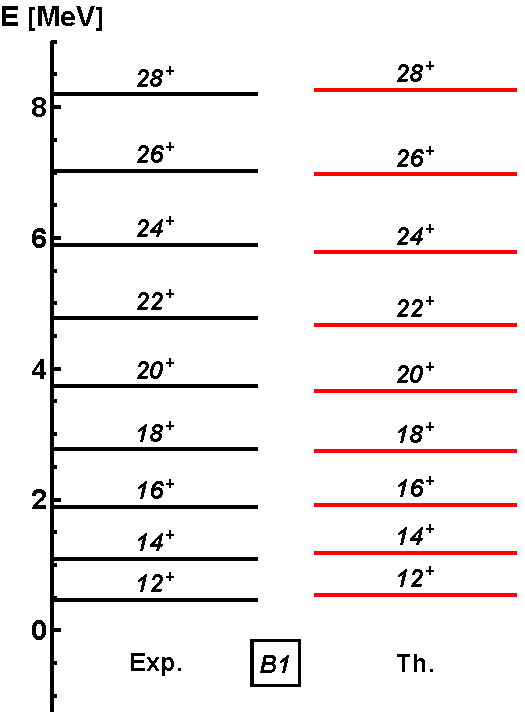
\includegraphics[scale=0.3]{Figs/ba130-band1.pdf}
      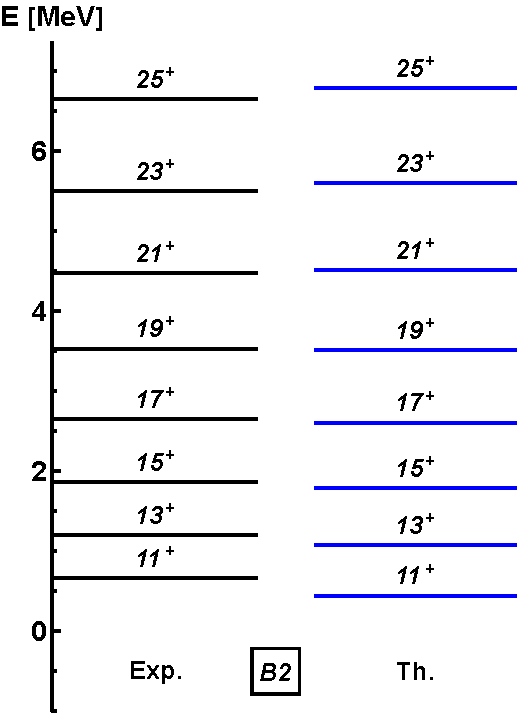
\includegraphics[scale=0.3]{Figs/ba130-band2.pdf}
      \tiny{\emph{Poenaru, 2022, unpublished}}
    \end{figure}
  \end{column}
\end{columns}
\end{frame}

\begin{frame}
  \frametitle{New Results for A=130 IV}
  \begin{itemize}
    \item \textbf{Left:} Wobbling energy* $E_\text{wob}(I)=E_\text{B2}(I)-E_\text{B1}(I)$
    \item \textbf{Center:} Rotational frequency $\hbar\omega_\text{rot}$ - collective
    \item \textbf{Right:} Interband transition probabilities $I_\text{B2}\to I_\text{B1}$
  \end{itemize}
  \begin{figure}
    \centering
    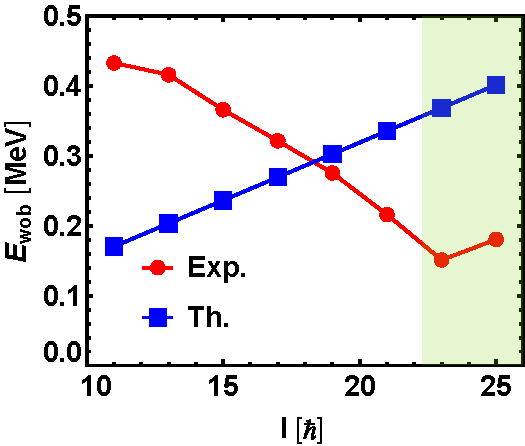
\includegraphics[scale=0.4]{Figs/ba130-wobbling-energies-edited.pdf}
    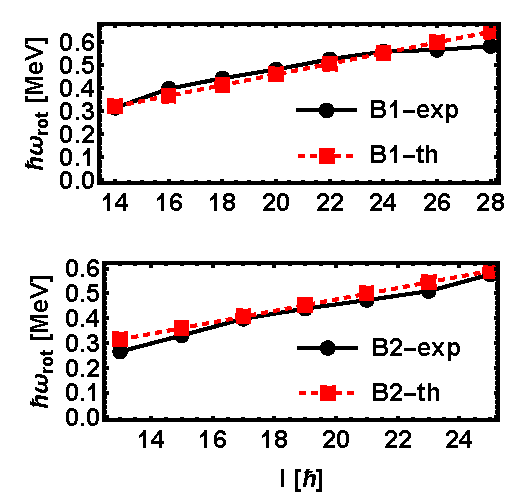
\includegraphics[scale=0.36]{Figs/ba130-rotational-frequencies.pdf}
    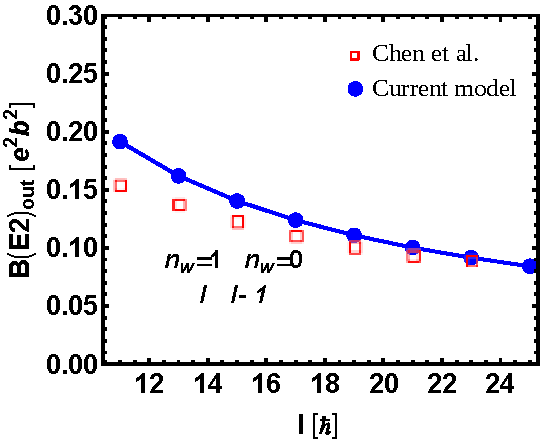
\includegraphics[scale=0.4]{Figs/ba130-EM.pdf}
    \tiny{\emph{Poenaru, 2022, unpublished}}
  \end{figure}
\end{frame}

\begin{frame}
  \frametitle{Electromagnetic transitions}
  \begin{columns}
    \begin{column}{0.72\textwidth}
      \begin{block}{Even-$A$ nuclei conclusions}
        \begin{itemize}
          \item $\beta=0.24$ and $\gamma=21.5^\circ$ were adopted for \emph{quadrupole moments} and \emph{transition probabilities}
          \item \par PRM values are calculated by Chen et al through a similar approach of minimizing the $\chi^2$-function
          \item Main rotation occurs along $3$-axis
          \item Approximation only reproduces $E_\text{wob}$ in the high-spin limit
        \end{itemize}
      \end{block}
    \end{column}
    \begin{column}{0.28\textwidth}
      \begin{table}
        \centering
        \resizebox{\textwidth}{!}{%
        \begin{tabular}{|c|ccc|}
          \hline
          \multirow{2}{*}{$I$} & \multicolumn{3}{c|}{$B(E2)_\text{out}/B(E2)_\text{in}$}                          \\ \cline{2-4} 
          & \multicolumn{1}{c|}{Th.} & \multicolumn{1}{c|}{PRM*} & Exp. \\ \hline
          11                   & \multicolumn{1}{c|}{0.37}       & \multicolumn{1}{c|}{-}           & -             \\ \hline
          13                   & \multicolumn{1}{c|}{0.32}       & \multicolumn{1}{c|}{0.51}       & 0.32         \\ \hline
          15                   & \multicolumn{1}{c|}{0.27}       & \multicolumn{1}{c|}{0.42}       & 0.36         \\ \hline
          17                   & \multicolumn{1}{c|}{0.24}       & \multicolumn{1}{c|}{0.35}       & 0.22         \\ \hline
          19                   & \multicolumn{1}{c|}{0.21}       & \multicolumn{1}{c|}{0.29}       & 0.22         \\ \hline
          21                   & \multicolumn{1}{c|}{0.19}       & \multicolumn{1}{c|}{0.25}       & 0.41         \\ \hline
          23                   & \multicolumn{1}{c|}{0.18}       & \multicolumn{1}{c|}{-}           &  -            \\ \hline
          25                   & \multicolumn{1}{c|}{0.16}       & \multicolumn{1}{c|}{-}           &  -            \\ \hline
        \end{tabular}%
        }
      \end{table}
      \tiny{\emph{Poenaru, 2022, unpublished}}
      \end{column}
\end{columns}
\end{frame}

\begin{frame}
  \frametitle{Wobbling Motion in Odd-Mass Nuclei}
  \begin{block}{Particle-Rotor-Model}
    \begin{itemize}
      \item The precessional motion of $\mathbf{I}=\mathbf{R}+\mathbf{j}$ is caused by the coupling of an \emph{even-$A$ triaxial core} + \emph{odd-particle}
      % \item The odd nucleon drives the system to large deformations ($\gamma$) and it stabilizes the shape
      \item System: {\color{red}[even-$A$ core]} + {\color{blue}[odd quasi-particle moving in a quadrupole deformed mean-field generated by the core]}
    \end{itemize}
  \end{block}
  {\small
  \begin{align}
    \hat{H}=&{\color{red}H_\text{core}}+{\color{blue}H_\text{sp}}={\color{red}\sum_{k=1,2,3}\frac{1}{2\mathcal{J}_k}\left(\hat{I}_k-\hat{j}_k\right)^2}+\nonumber\\
            &+{\color{blue}\epsilon_j+\frac{V}{j(j+1)}\left[\cos\gamma\left(3\hat{j}_3^2-j^2\right)-\sqrt{3}\sin\gamma\left(\hat{j}_1^2-\hat{j}_2^2\right)\right]}
  \end{align}}%
  % \par{\tiny\textbf{Solving the Hamiltonian in semi-classical approach}}
  \par{\tiny\textbf{for $^{163}Lu$}: \textit{R Poenaru, AA Raduta, IJMPE, 2021}.}
  \par{\tiny\textbf{for $^{167}Pr$}: \textit{A. A. Raduta and R. Poenaru, Phys Rev C, 2020}.}
  \par{\tiny\textbf{for $^{135}Pr$}: \textit{A. A. Raduta and R. Poenaru, Journal of Physics G, 2020}.}
  % \fontsize{0.2cm}{0.2cm}\selectfont sss
\end{frame}

\begin{frame}
  \frametitle{Classical energy}
      \begin{block}{Energy spectrum for odd mass nuclei}
        \begin{itemize}
          \item Total energy is given in terms of \textbf{two wobbling frequencies}: $\Omega_1\to$ {\color{red}core} and $\Omega_2\to$ {\color{blue}odd-particle}
          % \item The frequencies represent the harmonic-like behavior of the wobbling motion in odd-$A$ nuclei
        \end{itemize}
        \begin{align}
          E_I&={\color{black}\epsilon_{j}}+{\color{black}\mathcal{H}_\text{min}(I)}+{\color{red}\hbar\Omega_1^I\left(n_{w_1}+\frac{1}{2}\right)}+{\color{blue}\hbar\Omega_2^I\left(n_{w_2}+\frac{1}{2}\right)}\nonumber
        \end{align} 
      \end{block}
  \begin{figure}
    \centering
    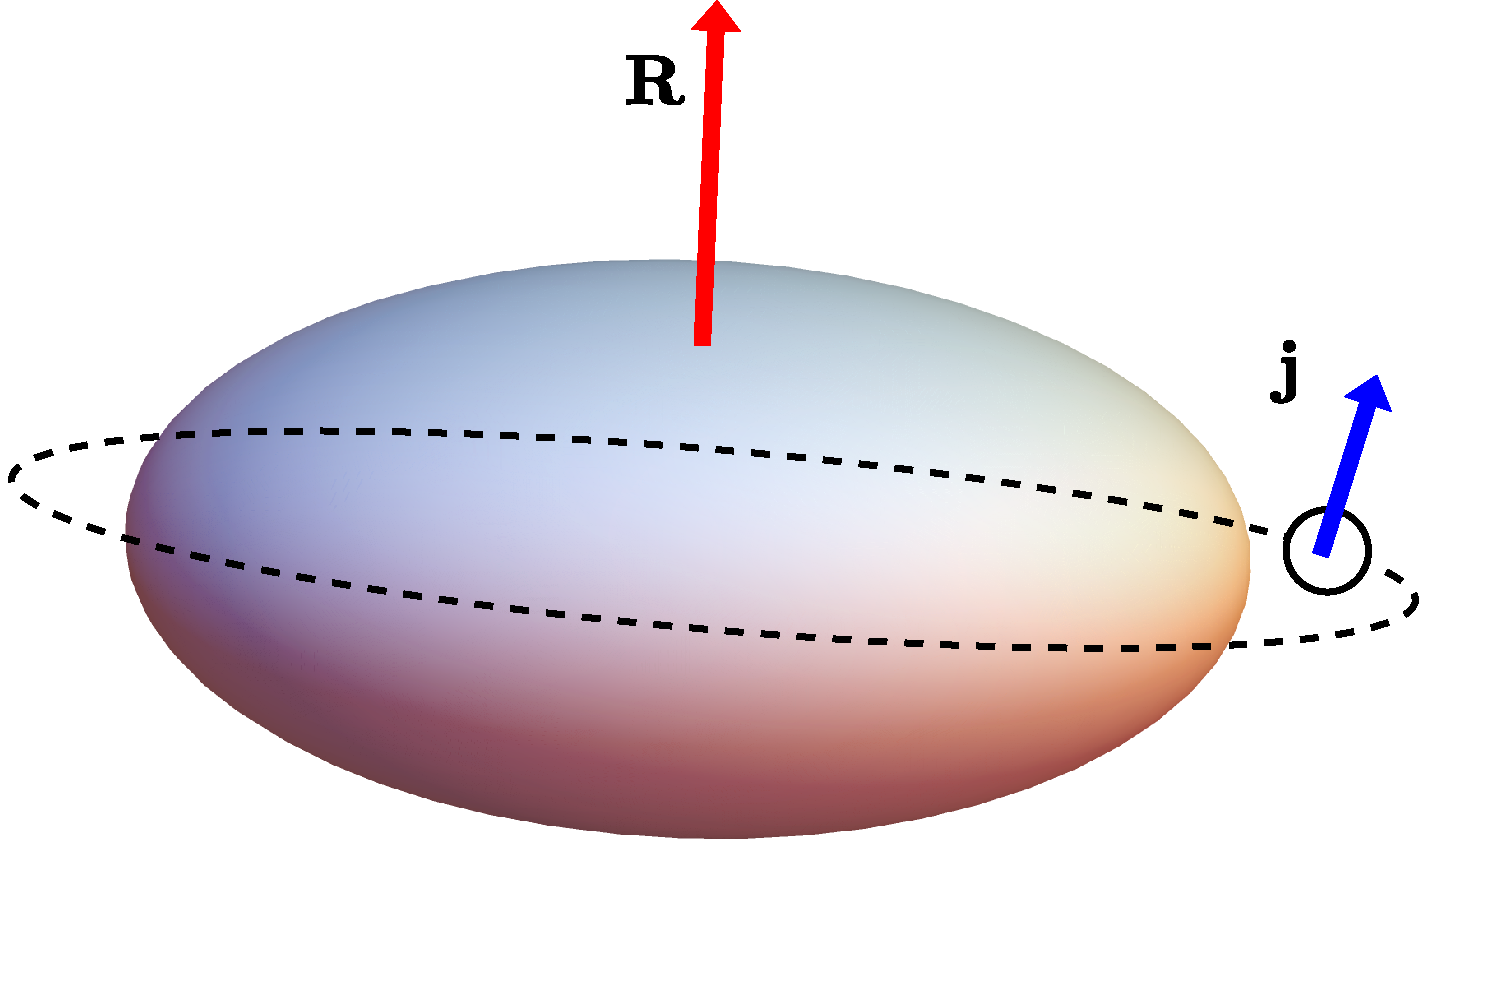
\includegraphics[scale=0.23]{Figs/triaxial-shapes-oddA.pdf}
  \end{figure}
\end{frame}

\begin{frame}
  \frametitle{Results for A=163}
  \begin{exampleblock}{Wobbling Motion in $^{163}$Lu}
    \begin{itemize}
      \item Four wobbling bands TSD1,2,3,4
      \item Stable minimum at $\beta=0.38$ and $\gamma=20^\circ$
    \end{itemize}
    \end{exampleblock}
  \begin{alertblock}{Model parametrization}
    \begin{itemize}
      \item 5 free parameters: $\mathcal{P}_\text{fit}=\{\mathcal{J}_1,\mathcal{J}_2,\mathcal{J}_3,V,\gamma\}$
      \item $\gamma^\text{fit}=22^\circ$ $\rightarrow$ $\gamma^\text{exp}=20^\circ$
      \item $V^\text{fit}=2.1\text{MeV}$ (literature: $0<V<8\ \text{MeV}$)
      \item the odd proton $i_{13/2}$ of positive parity couples to the triaxial core and generates TSD1,2,3,4
    \end{itemize}
  \end{alertblock}
    \begin{table}
      \centering
      \begin{tabular}{|c|c|c|c|}
      \hline
      $\mathcal{J}_1^\text{fit}$ & $\mathcal{J}_2^\text{fit}$ & $\mathcal{J}_3^\text{fit}$ & \multirow{2}{*}{$\left[\hbar^2\text{MeV}^{-1}\right]$} \\ \cline{1-3}
      $\mathbf{72}$                         & 15                         & 7                         &                                                       \\ \hline
      \end{tabular}
    \end{table}
    \tiny{R Poenaru, AA Raduta, IJMPE, 2021}
\end{frame}

\begin{frame}
  \frametitle{Results for A=163 II}
  \begin{figure}
    \centering
    \begin{minipage}{.5\textwidth}
      \centering
      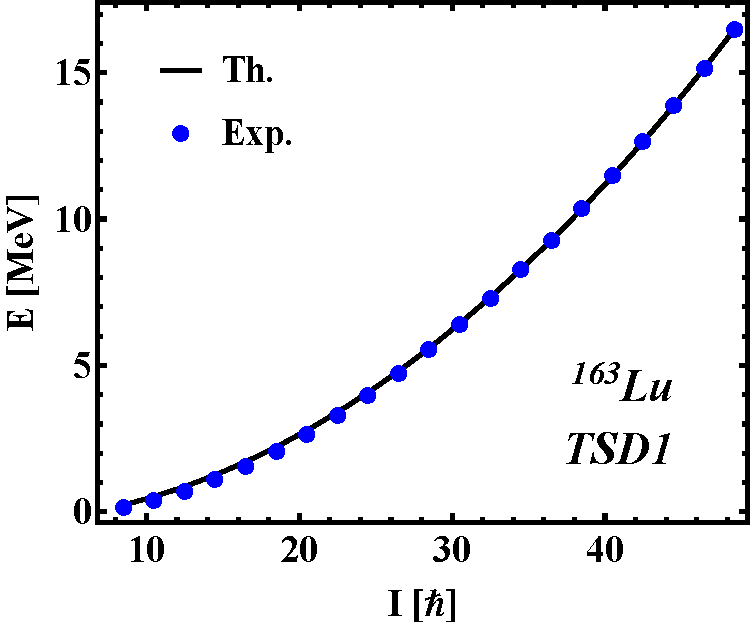
\includegraphics[scale=0.3]{figs/DoubleShift_TSD1.pdf}
      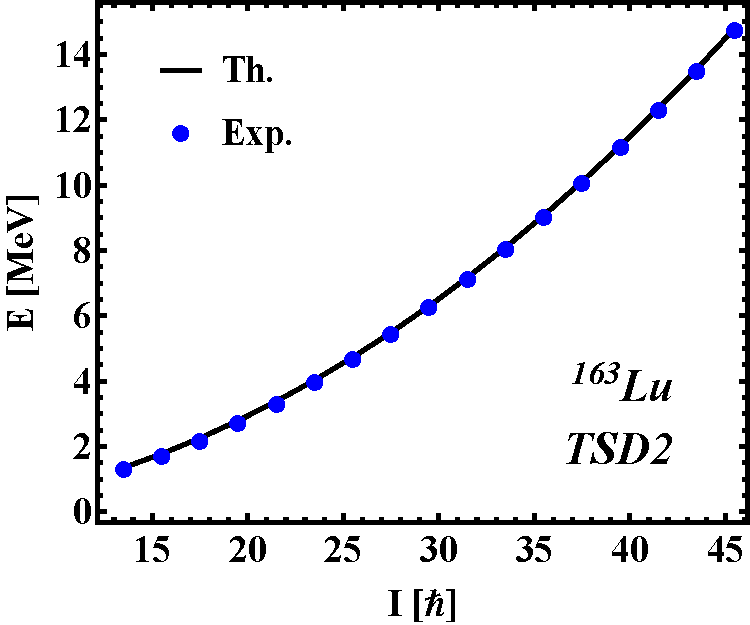
\includegraphics[scale=0.3]{figs/DoubleShift_TSD2.pdf}
    \end{minipage}%
    \begin{minipage}{.5\textwidth}
      \centering
     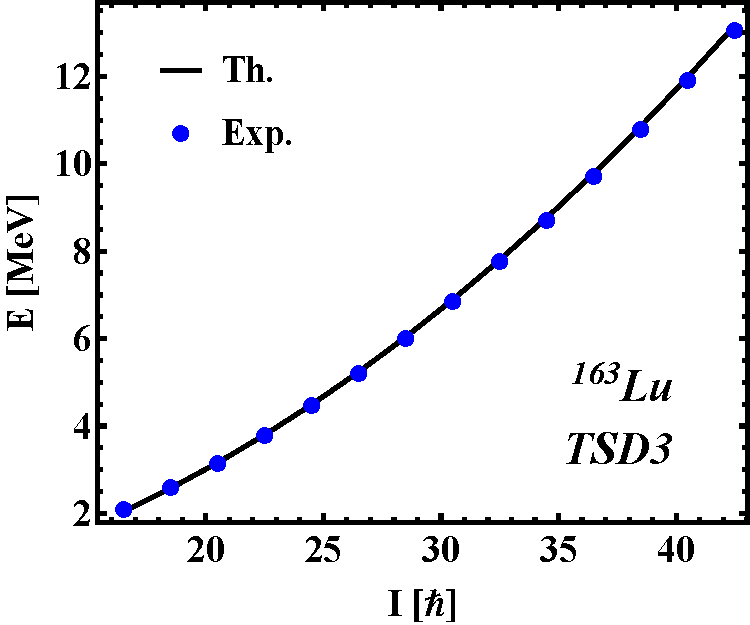
\includegraphics[scale=0.3]{figs/DoubleShift_TSD3.pdf}
     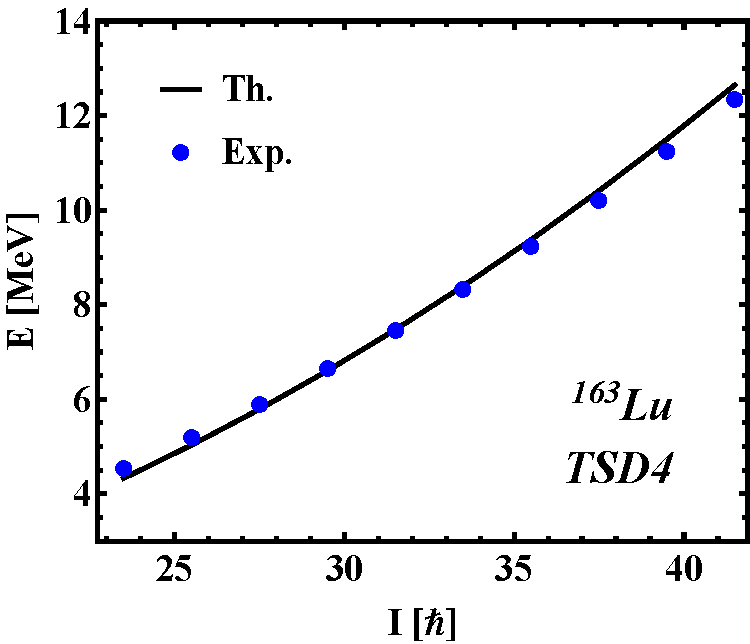
\includegraphics[scale=0.3]{figs/DoubleShift_TSD4.pdf}
    \end{minipage}
    \end{figure}
    \tiny{\emph{R Poenaru, AA Raduta - Rom. J. of Phys,66 (7-8), 2021}}
\end{frame}

\begin{frame}
  \frametitle{Results for A=163 III}
  \begin{itemize}
    \item Energy and angular momentum: constants of motion
    \begin{align}
      E=&\mathcal{S}_1x_1^2+\mathcal{S}_2x_2^2+\mathcal{S}_3x_3^2+\mathcal{S}_0^\text{core+sp}\ ,\\
      I^2=&x_1^2+x_2^2+x_3^2\ .
  \end{align}
  \end{itemize}
  \begin{figure}
    \centering
      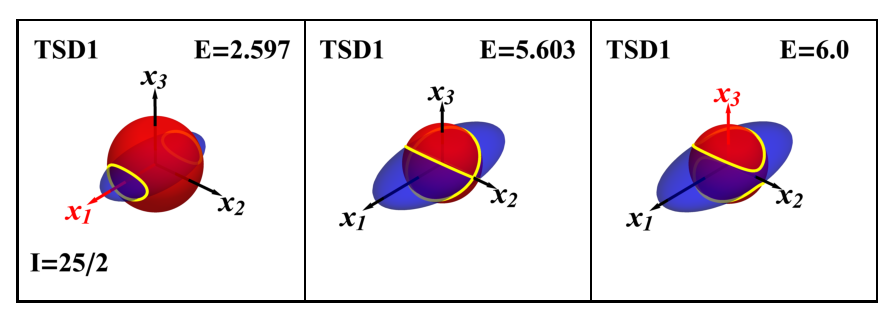
\includegraphics[scale=0.5]{figs/tsd1_spin1.eps}
      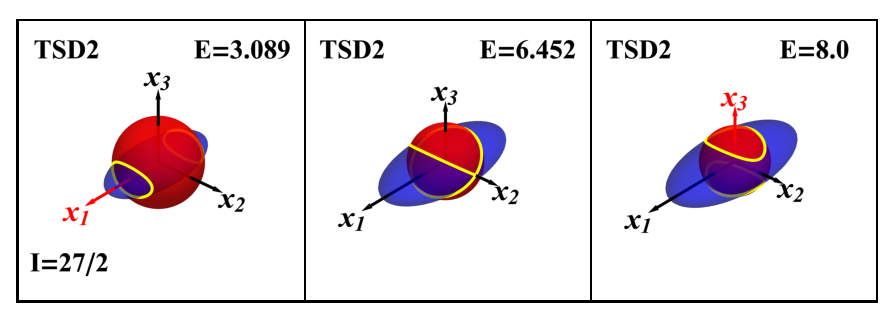
\includegraphics[scale=0.5]{figs/tsd2_spin1.eps}
    \end{figure}
    \tiny{\emph{R Poenaru, AA Raduta - Rom. J. of Phys,66 (9-10), 2021}}
\end{frame}

\begin{frame}
  \frametitle{Conclusions}
  \begin{itemize}
    \item Energy spectrum for even-even nuclei was obtained using a \emph{harmonic approximation}
    \item Energy spectrum for odd-$A$ nuclei was obtained using \emph{PRM}
    \item 1 oscillatory motion for even-$A$ $\longrightarrow\ \hbar\omega_\text{wob}$
    \item 2 oscillatory motions for odd-$A$ $\longrightarrow\ \hbar\Omega_{1,2}$
    \item odd-$A$: $\gamma$ obtained self-consistently (agreement with exp.)
    \item geometrical interpretations: consistent with quantal studies (\emph{Lawrie et al. 2020})
  \end{itemize}
\end{frame}

\begin{frame}
  \frametitle{Chart of wobblers}
  \begin{figure}
    \centering
    \begin{minipage}{.5\textwidth}
      \begin{figure}
        \centering
        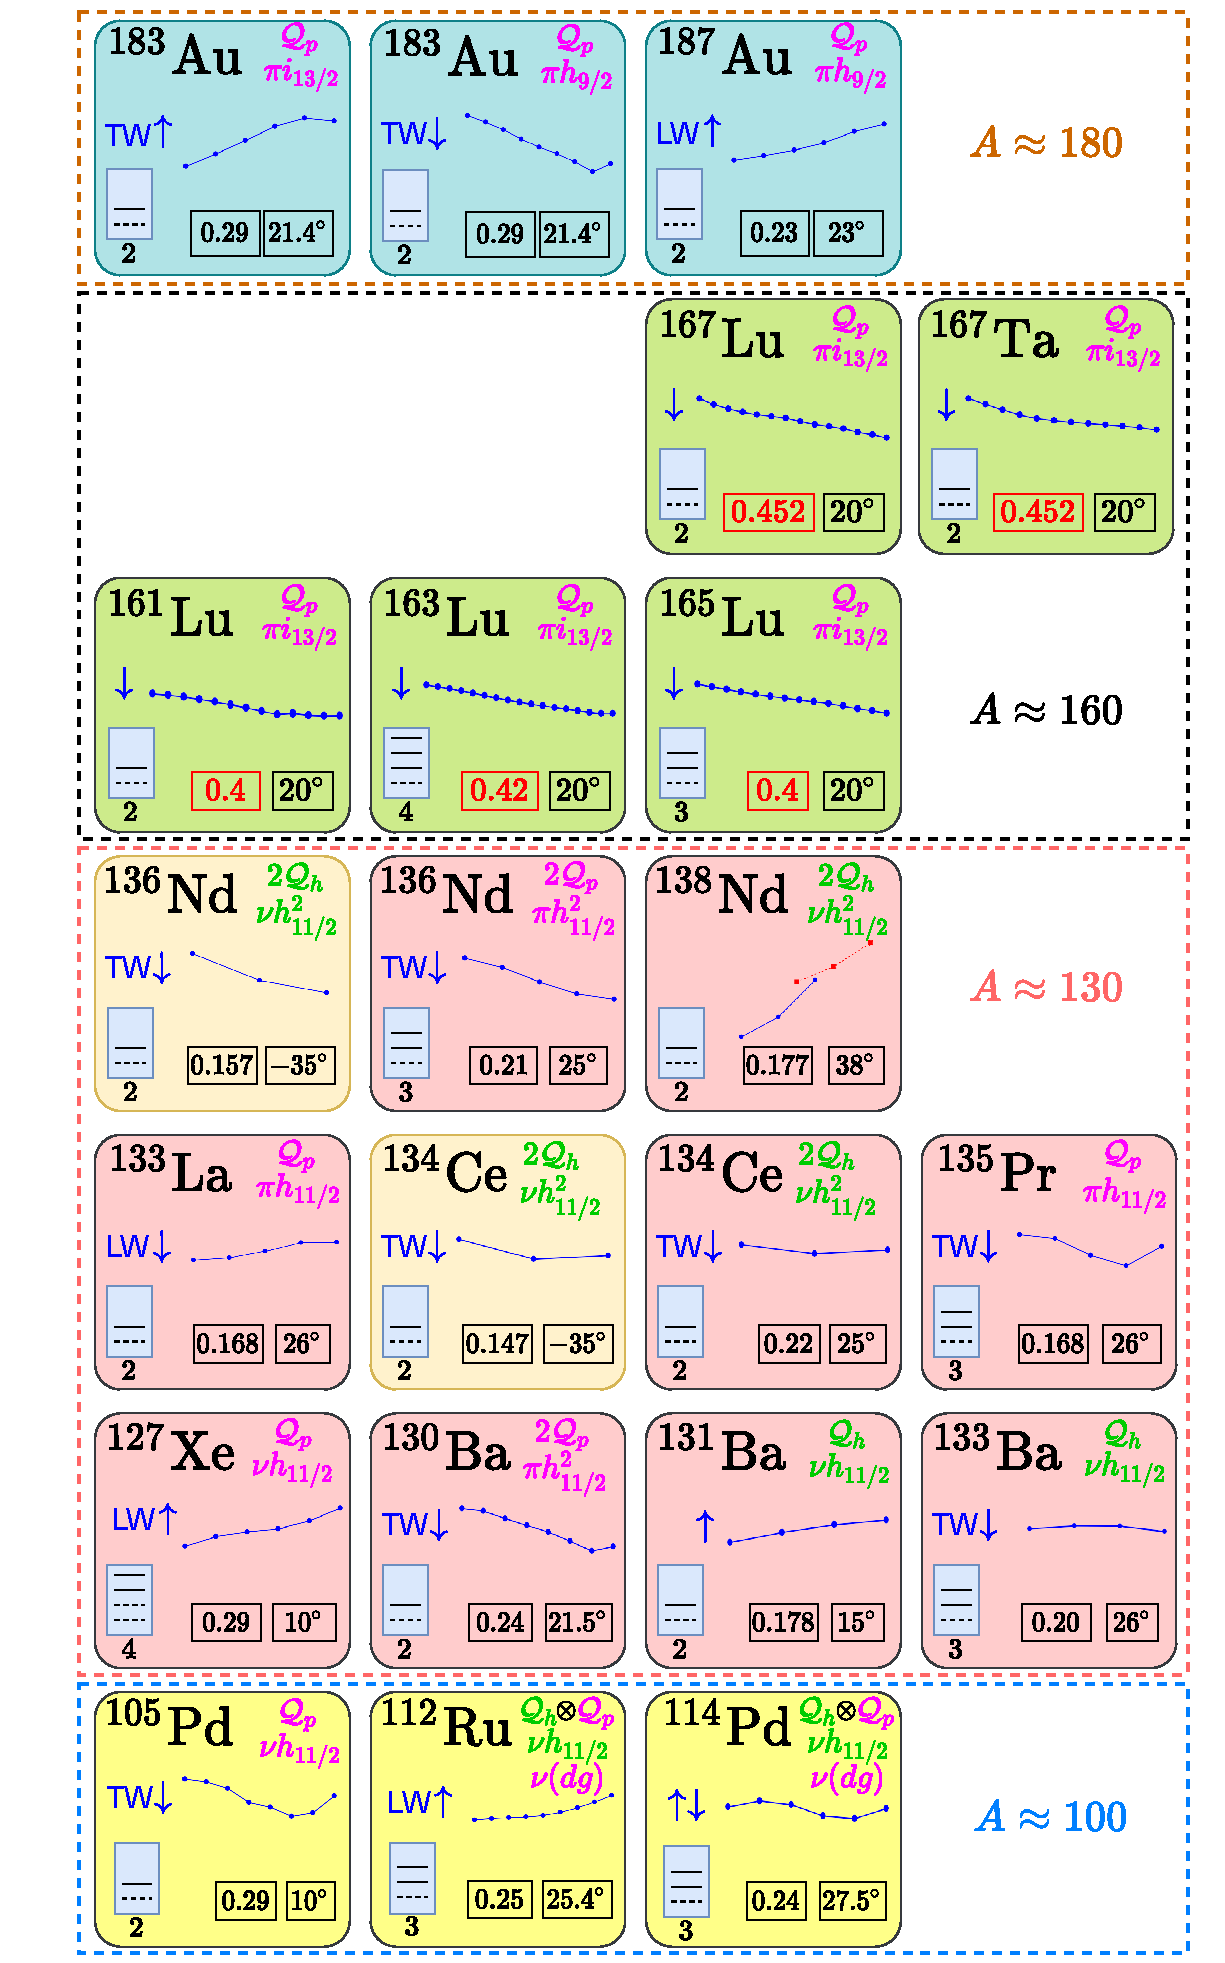
\includegraphics[scale=0.22]{Figs/wobblers-chart.pdf}
      \end{figure}
    \end{minipage}%
    \begin{minipage}{.5\textwidth}
      \par{\large{Thank you for your attention!}}
      \vspace*{3cm}
      \par{\tiny{Wobbling nuclei (up to date)}}
      \par{\tiny{Poenaru, 2022, in progress}}
    \end{minipage}
    \end{figure}
\end{frame}

%---------------------------------------------------------
\end{document}
%---------------------------------------------------------

% \begin{frame}
%   \frametitle{Highlighting text}
  
%   In this slide, some important text will be
%   \alert{highlighted} because it's important.
%   Please, don't abuse it.
  
%   \begin{block}{Remark}
%     Sample text
%   \end{block}
  
%   \begin{alertblock}{Important theorem}
%     Sample text in red box
%   \end{alertblock}
  
%   \begin{examples}
%     Sample text in green box. The title of the block is ``Examples".
%   \end{examples}
% \end{frame}